\documentclass[11pt]{article}
\usepackage[margin=0.75in]{geometry}
\usepackage{tikz}
\usepackage{amsmath}
\usepackage{amssymb}
% \usepackage{xcolor}
\usepackage{enumitem}
\usetikzlibrary{arrows.meta, patterns, positioning}

\usepackage[dvipsnames]{xcolor}

% Custom colors
\definecolor{carrierred}{RGB}{200,30,30}
\definecolor{sbplus}{RGB}{220,120,0}
\definecolor{sbminus}{RGB}{210,80,150}

\begin{document}

\begin{center}
    \textbf{In-class Tutorial: Coupled Cavities (Part 1)}\\
    March 23, 2026\\
    Lasers and Optomechanics\\~\\
    Name: \underline{\hspace{10cm}}
\end{center}


\noindent
\textbf{Coupled Cavity}\\
A \textit{coupled cavity} is a useful interferometer configuration for vastly enhancing the input power of a laser.
Advanced LIGO employs this configuration for the \textit{common-arm cavity} (CARM), 
by using a \textit{power-recycling mirror} (PRM) in front of the Fabry-Perot arms 
to recycle the light reflected by the Michelson back into the arms.

The difficulty in a coupled cavity comes in the two degrees of freedom it possesses, $L_1$ and $L_2$.
Sensing both $L_1$ and $L_2$ at the same time can be nontrivial.
This is why the RF sidebands are typically set to co-resonate inside the first cavity, but not the second.
In this tutorial, we will explore how a coupled cavity works.



\begin{center}
  
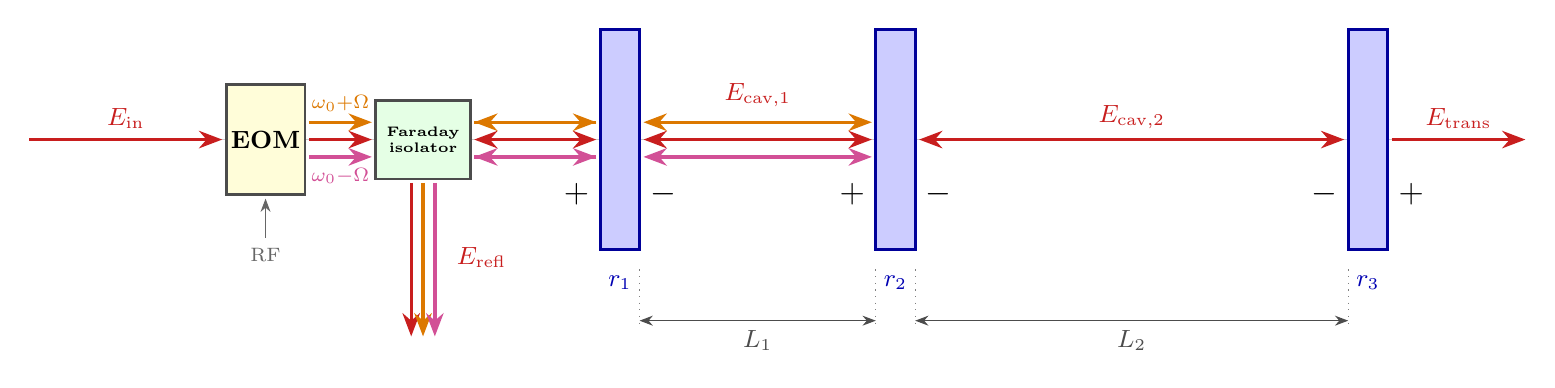
\begin{tikzpicture}[
    >=Stealth,
    thick,
    carrier/.style={->, very thick, carrierred},
    sbp/.style={->, very thick, sbplus},
    sbm/.style={->, very thick, sbminus},
]

%--- Coordinates ---
\def\rIx{0}         % r1 center x (input coupler)
\def\rIIx{3.5}      % r2 center x (coupling mirror)
\def\rIIIx{9.5}     % r3 center x (end mirror)
\def\mirH{1.4}      % half-height of mirrors
\def\mirW{0.25}     % half-width of mirror rectangles
% EOM box
\def\EOMx{-4.5}     % EOM center x
\def\EOMw{0.5}      % EOM half-width
\def\EOMh{0.7}      % EOM half-height
% Faraday isolator
\def\FIx{-2.5}      % FI center x
\def\FIy{0}
\def\FIw{0.6}       % FI half-width
\def\FIh{0.5}       % FI half-height
% Reflected beam drop
\def\Yrefl{-2.5}    % y level for downward E_refl exit

%--- Cavity axis (thin guide line) ---
\draw[gray!40, thin] (-7.5, 0) -- (\rIIIx+2.0, 0);

%============================================================
% EOM
%============================================================
\filldraw[fill=yellow!15!white, draw=black!70, line width=1pt]
    (\EOMx-\EOMw, -\EOMh) rectangle (\EOMx+\EOMw, \EOMh);
\node[font=\small\bfseries] at (\EOMx, 0) {EOM};
\draw[->, thin, black!60] (\EOMx, -\EOMh-0.55) -- (\EOMx, -\EOMh-0.05)
    node[below, font=\scriptsize, pos=0] {RF};

%============================================================
% Faraday isolator
%============================================================
\filldraw[fill=green!10!white, draw=black!70, line width=1pt]
    (\FIx-\FIw, \FIy-\FIh) rectangle (\FIx+\FIw, \FIy+\FIh);
\node[font=\tiny\bfseries, align=center] at (\FIx, \FIy) {Faraday\\isolator};

%============================================================
% Input beam: single carrier, left to EOM
%============================================================
\draw[carrier] (-7.5, 0) -- (\EOMx-\EOMw-0.05, 0)
    node[midway, above, font=\small] {$E_\mathrm{in}$};

%============================================================
% EOM to Faraday isolator: carrier + sidebands
%============================================================
\draw[carrier] (\EOMx+\EOMw+0.05, 0) -- (\FIx-\FIw-0.05, 0);
\draw[sbp] (\EOMx+\EOMw+0.05,  0.22) -- (\FIx-\FIw-0.05,  0.22)
    node[midway, above, font=\scriptsize] {$\omega_0{+}\Omega$};
\draw[sbm] (\EOMx+\EOMw+0.05, -0.22) -- (\FIx-\FIw-0.05, -0.22)
    node[midway, below, font=\scriptsize] {$\omega_0{-}\Omega$};

%============================================================
% Faraday isolator to r1: double-headed carrier + sidebands
%============================================================
\draw[carrier, {Stealth}-{Stealth}] (\FIx+\FIw+0.05, 0) -- (\rIx-\mirW-0.05, 0);
\draw[sbp] (\FIx+\FIw+0.05,  0.22) -- (\rIx-\mirW-0.05,  0.22);
\draw[sbm] (\FIx+\FIw+0.05, -0.22) -- (\rIx-\mirW-0.05, -0.22);

%============================================================
% r1 -- input coupler
%============================================================
\filldraw[fill=blue!20!white, draw=blue!60!black, line width=1.2pt]
    (\rIx-\mirW, -\mirH) rectangle (\rIx+\mirW, \mirH);
\node[below, blue!70!black, font=\small] at (\rIx, -\mirH-0.2) {$r_1$};
\node[font=\large, black] at (\rIx-\mirW-0.3, -0.7) {$+$};
\node[font=\large, black] at (\rIx+\mirW+0.3, -0.7) {$-$};

%============================================================
% Cavity 1 (r1 to r2): carrier + sidebands all resonate here
%============================================================
\draw[carrier, {Stealth}-{Stealth}] (\rIx+\mirW+0.05, 0) -- (\rIIx-\mirW-0.05, 0)
    node[midway, above=8pt, font=\small] {$E_\mathrm{cav,1}$};
\draw[sbp, {Stealth}-{Stealth}] (\rIx+\mirW+0.05,  0.22) -- (\rIIx-\mirW-0.05,  0.22);
\draw[sbm, {Stealth}-{Stealth}] (\rIx+\mirW+0.05, -0.22) -- (\rIIx-\mirW-0.05, -0.22);

%============================================================
% r2 -- coupling mirror (HR sides face both cavities)
%============================================================
\filldraw[fill=blue!20!white, draw=blue!60!black, line width=1.2pt]
    (\rIIx-\mirW, -\mirH) rectangle (\rIIx+\mirW, \mirH);
\node[below, blue!70!black, font=\small] at (\rIIx, -\mirH-0.2) {$r_2$};
\node[font=\large, black] at (\rIIx-\mirW-0.3, -0.7) {$+$};
\node[font=\large, black] at (\rIIx+\mirW+0.3, -0.7) {$-$};

%============================================================
% Cavity 2 (r2 to r3): carrier only, sidebands do not enter
%============================================================
\draw[carrier, {Stealth}-{Stealth}] (\rIIx+\mirW+0.05, 0) -- (\rIIIx-\mirW-0.05, 0)
    node[midway, above, font=\small] {$E_\mathrm{cav,2}$};

%============================================================
% r3 -- end mirror
%============================================================
\filldraw[fill=blue!20!white, draw=blue!60!black, line width=1.2pt]
    (\rIIIx-\mirW, -\mirH) rectangle (\rIIIx+\mirW, \mirH);
\node[below, blue!70!black, font=\small] at (\rIIIx, -\mirH-0.2) {$r_3$};
\node[font=\large, black] at (\rIIIx-\mirW-0.3, -0.7) {$-$};
\node[font=\large, black] at (\rIIIx+\mirW+0.3, -0.7) {$+$};

%============================================================
% Transmitted beam: carrier only exiting right of r3
%============================================================
\draw[carrier] (\rIIIx+\mirW+0.05, 0) -- (\rIIIx+2.0, 0)
    node[midway, above, font=\small] {$E_\mathrm{trans}$};

%============================================================
% Reflected beams: sidebands from r1 back to FI, then drop down
%============================================================
\draw[sbp] (\rIx-\mirW-0.05,  0.22) -- (\FIx+\FIw+0.05,  0.22);
\draw[sbm] (\rIx-\mirW-0.05, -0.22) -- (\FIx+\FIw+0.05, -0.22);

% Downward exits from bottom of Faraday isolator
\draw[carrier] (\FIx-0.15, -\FIh-0.05) -- (\FIx-0.15, \Yrefl);
\draw[sbp]     (\FIx,      -\FIh-0.05) -- (\FIx,      \Yrefl);
\draw[sbm]     (\FIx+0.15, -\FIh-0.05) -- (\FIx+0.15, \Yrefl);
\node[right, font=\small, carrierred] at (\FIx+0.15+0.15, {0.5*(-\FIh+\Yrefl)}) {$E_\mathrm{refl}$};
% \draw[carrier] (\FIx+0.15+0.15) -- (0.5*(-\FIh+\Yrefl))
%     node[right, font=\small] {$E_\mathrm{refl}$};

%============================================================
% Dimension annotations
%============================================================
% L1: r1 right face to r2 left face
\draw[<->, thin, black!70]
    (\rIx+\mirW, -\mirH-0.9) -- (\rIIx-\mirW, -\mirH-0.9)
    node[midway, below, font=\small] {$L_1$};
\draw[dotted, thin, gray] (\rIx+\mirW,  -\mirH-0.25) -- (\rIx+\mirW,  -\mirH-1.0);
\draw[dotted, thin, gray] (\rIIx-\mirW, -\mirH-0.25) -- (\rIIx-\mirW, -\mirH-1.0);

% L2: r2 right face to r3 left face
\draw[<->, thin, black!70]
    (\rIIx+\mirW, -\mirH-0.9) -- (\rIIIx-\mirW, -\mirH-0.9)
    node[midway, below, font=\small] {$L_2$};
\draw[dotted, thin, gray] (\rIIx+\mirW,  -\mirH-0.25) -- (\rIIx+\mirW,  -\mirH-1.0);
\draw[dotted, thin, gray] (\rIIIx-\mirW, -\mirH-0.25) -- (\rIIIx-\mirW, -\mirH-1.0);

\end{tikzpicture}

\vspace{0.5cm}

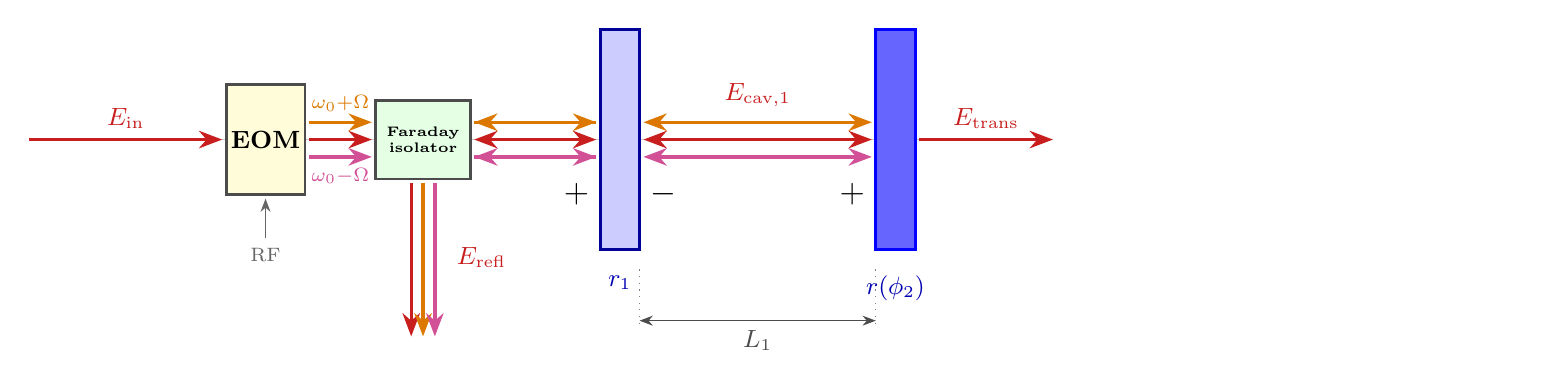
\begin{tikzpicture}[
    >=Stealth,
    thick,
    carrier/.style={->, very thick, carrierred},
    sbp/.style={->, very thick, sbplus},
    sbm/.style={->, very thick, sbminus},
]

%--- Coordinates ---
\def\rIx{0}         % r1 center x (input coupler)
\def\rIIx{3.5}      % r2 center x (end mirror, aligned with r2 above)
\def\mirH{1.4}      % half-height of mirrors
\def\mirW{0.25}     % half-width of mirror rectangles
% EOM box
\def\EOMx{-4.5}     % EOM center x
\def\EOMw{0.5}      % EOM half-width
\def\EOMh{0.7}      % EOM half-height
% Faraday isolator
\def\FIx{-2.5}      % FI center x
\def\FIy{0}
\def\FIw{0.6}       % FI half-width
\def\FIh{0.5}       % FI half-height
% Reflected beam drop
\def\Yrefl{-2.5}    % y level for downward E_refl exit

%--- Cavity axis (thin guide line) ---
\draw[gray!40, thin] (-7.5, 0) -- (\rIIx+2.0, 0);

%============================================================
% EOM
%============================================================
\filldraw[fill=yellow!15!white, draw=black!70, line width=1pt]
    (\EOMx-\EOMw, -\EOMh) rectangle (\EOMx+\EOMw, \EOMh);
\node[font=\small\bfseries] at (\EOMx, 0) {EOM};
\draw[->, thin, black!60] (\EOMx, -\EOMh-0.55) -- (\EOMx, -\EOMh-0.05)
    node[below, font=\scriptsize, pos=0] {RF};

%============================================================
% Faraday isolator
%============================================================
\filldraw[fill=green!10!white, draw=black!70, line width=1pt]
    (\FIx-\FIw, \FIy-\FIh) rectangle (\FIx+\FIw, \FIy+\FIh);
\node[font=\tiny\bfseries, align=center] at (\FIx, \FIy) {Faraday\\isolator};

%============================================================
% Input beam: single carrier, left to EOM
%============================================================
\draw[carrier] (-7.5, 0) -- (\EOMx-\EOMw-0.05, 0)
    node[midway, above, font=\small] {$E_\mathrm{in}$};

%============================================================
% EOM to Faraday isolator: carrier + sidebands
%============================================================
\draw[carrier] (\EOMx+\EOMw+0.05, 0) -- (\FIx-\FIw-0.05, 0);
\draw[sbp] (\EOMx+\EOMw+0.05,  0.22) -- (\FIx-\FIw-0.05,  0.22)
    node[midway, above, font=\scriptsize] {$\omega_0{+}\Omega$};
\draw[sbm] (\EOMx+\EOMw+0.05, -0.22) -- (\FIx-\FIw-0.05, -0.22)
    node[midway, below, font=\scriptsize] {$\omega_0{-}\Omega$};

%============================================================
% Faraday isolator to r1: double-headed carrier + sidebands
%============================================================
\draw[carrier, {Stealth}-{Stealth}] (\FIx+\FIw+0.05, 0) -- (\rIx-\mirW-0.05, 0);
\draw[sbp] (\FIx+\FIw+0.05,  0.22) -- (\rIx-\mirW-0.05,  0.22);
\draw[sbm] (\FIx+\FIw+0.05, -0.22) -- (\rIx-\mirW-0.05, -0.22);

%============================================================
% r1 -- input coupler
%============================================================
\filldraw[fill=blue!20!white, draw=blue!60!black, line width=1.2pt]
    (\rIx-\mirW, -\mirH) rectangle (\rIx+\mirW, \mirH);
\node[below, blue!70!black, font=\small] at (\rIx, -\mirH-0.2) {$r_1$};
\node[font=\large, black] at (\rIx-\mirW-0.3, -0.7) {$+$};
\node[font=\large, black] at (\rIx+\mirW+0.3, -0.7) {$-$};

%============================================================
% Cavity (r1 to r2): carrier + sidebands
%============================================================
\draw[carrier, {Stealth}-{Stealth}] (\rIx+\mirW+0.05, 0) -- (\rIIx-\mirW-0.05, 0)
    node[midway, above=8pt, font=\small] {$E_\mathrm{cav,1}$};
\draw[sbp, {Stealth}-{Stealth}] (\rIx+\mirW+0.05,  0.22) -- (\rIIx-\mirW-0.05,  0.22);
\draw[sbm, {Stealth}-{Stealth}] (\rIx+\mirW+0.05, -0.22) -- (\rIIx-\mirW-0.05, -0.22);

%============================================================
% r2 -- end mirror (compound: represents r2+r3 as complex reflectivity)
%============================================================
\filldraw[fill=blue!60!white, draw=blue!100!black, line width=1.2pt]
    (\rIIx-\mirW, -\mirH) rectangle (\rIIx+\mirW, \mirH);
\node[font=\large, black] at (\rIIx-\mirW-0.3, -0.7) {$+$};
\node[below, blue!70!black, font=\small] at (\rIIx, -\mirH-0.2) {$r(\phi_2)$};

%============================================================
% Transmitted beam: exiting right of r2
%============================================================
\draw[carrier] (\rIIx+\mirW+0.05, 0) -- (\rIIx+2.0, 0)
    node[midway, above, font=\small] {$E_\mathrm{trans}$};

%============================================================
% Reflected beams: sidebands from r1 back to FI, then drop down
%============================================================
\draw[sbp] (\rIx-\mirW-0.05,  0.22) -- (\FIx+\FIw+0.05,  0.22);
\draw[sbm] (\rIx-\mirW-0.05, -0.22) -- (\FIx+\FIw+0.05, -0.22);

% Downward exits from bottom of Faraday isolator
\draw[carrier] (\FIx-0.15, -\FIh-0.05) -- (\FIx-0.15, \Yrefl);
\draw[sbp]     (\FIx,      -\FIh-0.05) -- (\FIx,      \Yrefl);
\draw[sbm]     (\FIx+0.15, -\FIh-0.05) -- (\FIx+0.15, \Yrefl);
\node[right, font=\small, carrierred] at (\FIx+0.15+0.15, {0.5*(-\FIh+\Yrefl)}) {$E_\mathrm{refl}$};

%============================================================
% Dimension annotation
%============================================================
% L1: r1 right face to r2 left face
\draw[<->, thin, black!70]
    (\rIx+\mirW, -\mirH-0.9) -- (\rIIx-\mirW, -\mirH-0.9)
    node[midway, below, font=\small] {$L_1$};
\draw[dotted, thin, gray] (\rIx+\mirW,  -\mirH-0.25) -- (\rIx+\mirW,  -\mirH-1.0);
\draw[dotted, thin, gray] (\rIIx-\mirW, -\mirH-0.25) -- (\rIIx-\mirW, -\mirH-1.0);

% Invisible path to match bounding box width of top diagram
\path (-7.5, 0) -- (11.5, 0);

\end{tikzpicture}
\end{center}

\noindent Figure 1A: Coupled-cavity interferometer, with three mirrors aligned and carrier plus one set of RF sidebands incident.\\
\noindent Figure 1B: Compound interferometer representing the coupled-cavity interferometer, where we have ``collapsed'' the $r_2$ and $r_3$ mirrors into a single mirror with reflectivity $r(\phi_2)$.

Recall the Fabry-Perot cavity reflection equation is 
\begin{align}
\label{eq:fp_refl}
r(\phi) &= \dfrac{E_\mathrm{refl}}{E_\mathrm{in}}(\phi) = \dfrac{r_i - r_e e^{-i 2 \phi}}{1 - r_i r_e e^{-i 2 \phi}}\\
\label{eq:fp_cav}
g(\phi) &= \dfrac{E_\mathrm{cav}}{E_\mathrm{in}}(\phi) = \dfrac{t_i}{1 - r_i r_e e^{-i 2 \phi}}\\
\label{eq:fp_trans}
t(\phi) &= \dfrac{E_\mathrm{trans}}{E_\mathrm{in}}(\phi) = \dfrac{t_i t_e e^{-i \phi}}{1 - r_i r_e e^{-i 2 \phi}}
\end{align} 
where $r_i, t_i$ and $r_e,t_e$ are the input and end mirror reflectivities and transmissions.

\newpage 
\noindent
\textbf{Compound Interferometers and Complex Reflectivities}\\

Above in Figure 1A, we have a diagram of a coupled cavity, featuring three aligned mirrors $r_1, r_2, r_3$.
Between $r_1$ and $r_2$ we have a length $L_1$, or a single-pass phase $\phi_1 = k L_1$.
Similarly, between $r_2$ and $r_3$ we accrue $\phi_2 = k L_2$.
Essentially, a coupled-cavity is just taking a Fabry-Perot interferometer and placing an additional mirror in front.  
In fact, we can simplify our thinking by using our understanding of the Fabry-Perot reflectivity $r(\phi)$.

Figure 1B shows a \textit{compound Fabry-Perot interferometer} representing our original coupled cavity.
The compound interferometer recognizes the Fabry-Perot interferometer inside the coupled-cavity, and ``collapses'' the two mirrors and fields inside into a single ``compound'' mirror, which we say has reflectivity $r(\phi_2)$ and transmission $t(\phi_2)$.
Equations~\ref{eq:fp_refl} and \ref{eq:fp_trans} shows our Fabry-Perot reflectivity and transmission, which describe the field reflected and transmitted by the compound mirror.


Below we will analyze the coupled cavity, 
calculate the \textit{arm gain} and \textit{power-recycling gain}, 
as well as calculate the \textit{coupled-cavity pole}.
In Part 2, we'll build a \textit{sensing matrix} for our two degrees of freedom $\phi_1$ and $\phi_2$.
I recommend using Mathematica, sympy, or Desmos to make some of these plots at the end.

\vspace{0.5cm}

\noindent
\textbf{Analysis of the Coupled Cavity}

We will focus only on the carrier $E_\mathrm{in} = E_0 e^{i \omega_0 t}$ analysis first.
The coupled-cavity typically resonates the carrier in both the first and second cavities.

\textcolor{MidnightBlue}{\textbf{1. Write the second cavity reflectivity, gain, and transmission expressions $$r(\phi_2), g(\phi_2), t(\phi_2),$$ using Equations~\ref{eq:fp_refl}, \ref{eq:fp_cav}, and \ref{eq:fp_trans}, in terms of $r_2,r_3, t_2, t_3,$ and $\phi_2$}}.

\textcolor{MidnightBlue}{\textbf{2. Write the compound cavity reflectivity, gain, and transmission expressions $$r(\phi_1,\phi_2), g_1(\phi_1,\phi_2), t(\phi_1,\phi_2),$$ in terms of $r_1,t_1,\phi_1$, and your expressions from (1)}}.\\
Here $g_1$ is used to emphasize this is the amplitude gain for the first cavity.

\textcolor{MidnightBlue}{\textbf{3. Expand out your terms for $r(\phi_1,\phi_2), g_1(\phi_1,\phi_2), t(\phi_1,\phi_2)$, to get the full expressions in terms of $r_1,r_2,r_3,t_1,t_2,t_3,\phi_1,\phi_2$}}.

\textcolor{MidnightBlue}{\textbf{4. How might you derive the amplitude gain for the second cavity $g_2(\phi_1,\phi_2)$?}}.

\textcolor{MidnightBlue}{\textbf{5. What should the phases for $\phi_1$ and $\phi_2$ be to maximize carrier power in the arm cavity?}}\\
In Advanced LIGO, the \textit{power-recycling gain} refers to the power gain experienced inside the first cavity $|g_1(\phi_1,\phi_2)|^2$, while the \textit{arm gain} is just the usual FP gain $g(\phi_2)$.
It can be useful to consider the arm cavity gain and reflectivity ($g(\phi_2)$ and $r(\phi_2)$) here.
You may need the fact that the end mirror transmission $T_3 = 5~\mathrm{ppm}$, while the middle mirror transmission $T_2 = 1.5~\%$.

\textcolor{MidnightBlue}{\textbf{6. What should the phases for $\phi_1$ and $\phi_2$ for the sidebands in the coupled cavity?}}
In Advanced LIGO, the RF sideband frequency $\Omega$ is selected such that the sidebands are \textit{anti-resonant} in the arms but resonant in the power-recycling cavity.

\textcolor{MidnightBlue}{\textbf{7. Find the coupled cavity pole $\omega_{cc}$ for carrier.}}\\
The \textit{coupled-cavity pole} $\omega_{cc}$ is used to describe the frequency response of the coupled cavity.
For simplicity, you will need to set the denominator of your coupled cavity field solutions to zero, and let $\phi_1 = 0$ and $\phi_2 = \omega_{cc} L_2 / c$.
In Advanced LIGO, the arm cavity's higher finesse and longer length let it's dynamics dominate over the first cavity, which is why $\phi_1 = 0$ is a decent approximation.





\end{document}